\documentclass[letterpaper,hyper]{THG_RFC}

% Path to figures, plots
\graphicspath{{./pics/}{./plots/}}

%% TikZ
\usepackage{tikz}
\usetikzlibrary{patterns, shapes, positioning, decorations.pathreplacing,
backgrounds, fit}
\usepackage{gnuplot-lua-tikz}

% SI units
%\usepackage{textcomp}
\usepackage[binary-units]{siunitx}
\sisetup{per-mode = symbol}
\providecommand{\gbps}[1]{\SI{#1}{\giga\byte\per\second}}
\providecommand{\mbps}[1]{\SI{#1}{\mega\byte\per\second}}
\providecommand{\gb}[1]{\SI{#1}{\giga\byte}}
\providecommand{\mb}[1]{\SI{#1}{\mega\byte}}
\providecommand{\kb}[1]{\SI{#1}{\kilo\byte}}

% Code snippets
\usepackage{listings}
\def\lstsetc{\lstset{language=C,
  numbers=left,
  xleftmargin=1.8em,
  frame=L,
  framexleftmargin=0.2em,
  rulecolor=\color{rulecolor},
  numberstyle=\tiny\color{gray},
  stepnumber=1,
  showspaces=false, 
  showstringspaces=false,
  breaklines=true,
  basicstyle=\footnotesize\ttfamily,
  stringstyle=\itshape,
  commentstyle=\itshape\bfseries,
  morekeywords={main, size_t, malloc, free,
    hsize_t, hid_t, herr_t, H5X_class_t, H5X_type_t, H5Q_combine_op_t,
    H5Q_type_t, H5Q_match_op_t,
    H5Fcreate, H5Fclose,
    H5Dcreate, H5Dopen, H5Dclose, H5Dwrite, H5Dread, H5Dquery,
    H5Qcreate, H5Qclose, H5Qcombine, H5Qget_type, H5Qget_match_op,
    H5Qget_components, H5Qget_combine_op, H5Qencode, H5Qdecode,
    H5Qapply,
    H5Screate_simple, H5Sclose, H5Sget_select_npoints,
    H5Xregister, H5Xunregister, H5Xcreate, H5Xremove, H5Xget_count, H5Xget_size,
    H5Xget_info
    }
  }
}

% Title, author, etc
\title{Data Analysis Extensions}
\author{Jerome Soumagne}
\author{Quincey Koziol}
\date{Oct 14, 2015}
\rfcversion{2014-07-17.v6}
\revision{Jul. 17, 2014}{Version 1 circulated for comment within The HDF Group.}
\revision{Aug. 20, 2014}{Version 2 circulated for comment within The HDF Group.}
\revision{Nov. 14, 2014}{Version 3 circulated for comment within The HDF Group.}
\revision{Feb. 25, 2015}{Version 4 edits and typo fixing.}
\revision{Jul. 24, 2015}{Version 5 edits to view object.}
\revision{Oct. 14, 2015}{Version 6 rework of query/view sections.}

%% Start the document
\begin{document}

%% Title
\maketitle

%% Abstract
\begin{abstract}
Accessing, selecting and retrieving data from an HDF5 container can be a time
consuming process, particularly so when data is very large. To enable, ease and 
accelerate this process, we introduce in this RFC extensions to the library
to efficiently query, select and index data.
\end{abstract}

\section{Introduction}
When working on large datasets, finding and selecting the interesting pieces of
the data can be a cumbersome process. Currently, the HDF5 library enables the 
application developer to select, read and write data but does not provide any 
mechanism to select and retrieve pieces without prior knowledge of their
content, or without the developer to provide the exact data coordinates that
he is willing to access. To satisfy that need, one must be able
to issue queries by specifying a data selection criteria. These queries,
when applied to the data, can then generate a selection, which contains the coordinates
that satisfy the query---this may imply accessing the data and selecting it,
depending on the query condition satisfaction. To accelerate and facilitate this
process (i.e., so that the data no longer needs to be directly accessed), one can
use indexing techniques, which consist of generating an index and using that index
to answer the query selection criteria and find the matching elements.

We define in this RFC the components that can enable application developers to
create complex and high-performance queries on both metadata and data elements
within an HDF5 container and retrieve the results of applying those query
operations. Support for these operations can be defined via:
\begin{itemize}
\item New \textit{query} objects\footnote{Query objects are
\textit{in-memory} objects, which therefore do not modify the content of the
container.\label{fn:object}} and API routines, enabling the construction of
query requests for execution on HDF5 containers;
\item New \textit{index} objects and API routines, which allows the creation of
indices on the contents of HDF5 containers, to improve query performance.
\end{itemize}

\section{Query Objects}
Query objects are the foundation of the data analysis operations in HDF5 and
can be built up from simple components in a programmatic way to create complex
operations using \textit{Boolean} operations. The current API is presented
below:

{\lstsetc
\begin{lstlisting}
hid_t  H5Qcreate(H5Q_type_t query_type, H5Q_match_op_t match_op, ...);
herr_t H5Qclose(hid_t query_id);
hid_t  H5Qcombine(hid_t query1_id, H5Q_combine_op_t combine_op, hid_t query2_id);
herr_t H5Qget_type(hid_t query_id, H5Q_type_t *query_type);
herr_t H5Qget_match_op(hid_t query_id, H5Q_match_op_t *match_op);
herr_t H5Qget_components(hid_t query_id, hid_t *subquery1_id, hid_t *subquery2_id);
herr_t H5Qget_combine_op(hid_t query_id, H5Q_combine_op_t *op_type);
herr_t H5Qencode(hid_t query_id, void *buf, size_t *nalloc);
hid_t  H5Qdecode(const void *buf);
\end{lstlisting}
}

\subsection{Query Creation}

The core query API is composed of
two routines: \texttt{H5Qcreate} and \texttt{H5Qcombine}. \texttt{H5Qcreate}
creates new queries, by specifying an aspect of an HDF5 container, such as:
\begin{itemize}
\item \texttt{H5Q\_TYPE\_DATA\_ELEM} (data element);
\item \texttt{H5Q\_TYPE\_LINK\_NAME} (link name);
\item \texttt{H5Q\_TYPE\_ATTR\_NAME} (attribute name);
\item \texttt{H5Q\_TYPE\_ATTR\_VALUE} (attribute value);
\end{itemize}
as well as a match operator, such as:
\begin{itemize}
\item \texttt{H5Q\_MATCH\_EQUAL} ($=$);
\item \texttt{H5Q\_MATCH\_NOT\_EQUAL} ($\neq$);
\item \texttt{H5Q\_MATCH\_LESS\_THAN} ($\leq$);
\item \texttt{H5Q\_MATCH\_GREATER\_THAN} ($\geq$);
\end{itemize}
and a value for the match operator.
Created query objects can be serialized and deserialized using the \texttt{H5Qencode}
and \texttt{H5Qdecode} routines\footnote{Serialization/deserialization of queries
were introduced so that queries can be sent through the network.}, and their
content can be retrieved using the corresponding accessor routines.
\texttt{H5Qcombine} combines two query objects into a
new query object, using boolean operators such as:
\begin{itemize}
\item \texttt{H5Q\_COMBINE\_AND} ($\mathrm{\land}$);
\item \texttt{H5Q\_COMBINE\_OR} ($\mathrm{\lor}$).
\end{itemize}
Queries created with \texttt{H5Qcombine} can be used as input to further
calls to \texttt{H5Qcombine}, creating more complex queries.

For example, a single call to \texttt{H5Qcreate} could create a query object
that would match data elements in any dataset within the container that are
equal to the value ``$\mathrm{17}$''. Another call to \texttt{H5Qcreate} could create a
query object that would match link names equal to ``$\mathrm{Pressure}$''.
Calling \texttt{H5Qcombine} with the $\mathrm{\land}$ operator and those two query
objects would create a new query object that matched elements equal to ``$\mathrm{17}$''
in HDF5 datasets with link names equal to ``$\mathrm{Pressure}$''.
Creating the data analysis extensions to HDF5 using a \textit{programmatic
interface} for defining queries avoids defining a text-based query language
as a core component of the data analysis interface, and is more in keeping with
the design and level of abstraction of the HDF5 API.
The HDF5 data model is more complex than traditional database tables and a
simpler query model would likely not be able to express the kinds of queries
needed to extract the full set of components of an HDF5 container. A text-based
query language (or GUI) could certainly be built on top of the query API
defined here to provide a more user-friendly (as opposed to
\textit{developer-friendly}) query syntax like ``$\mathrm{Pressure = 17}$''.
However, we regard this as out-of-scope for now.

\subsection{Query Execution and Views}
Applying a query to an HDF5 container creates an HDF5 \textit{view}. A view is
an anonymous HDF5 group in a temporary memory container. A view group contains up to
three 1-D dataset objects with references into the contents of the HDF5 container
that the query was applied to:
one with \textit{object} references, one with \textit{region} references and
one with \textit{attribute} references.

\begin{figure}
\tikzstyle{groupBox} = [draw, ellipse, fill=white, minimum size=20pt,
  text centered, font=\footnotesize\sffamily, text width=20pt, inner sep=0]

\tikzstyle{textBox} = [fill=white, inner sep=2pt, text centered, font=\footnotesize\sffamily]

\tikzstyle{link} = [->, thick, >=stealth', shorten <=1pt, shorten >=1pt]

\pgfmathsetseed{1}

\def\drawdataset#1{%
\begin{scope}[#1]
  \foreach \y in {-0.5} {
      \foreach \x in {-2.5,-1.5,-0.5,0.5,1.5} {
          \path[fill=white, draw] (\x,\y) rectangle ++(1,1);
      }
  }
\end{scope}
}

\begin{tikzpicture}

% View
\node[groupBox] (view) {/};

% Refs
\node[below=30pt of view, inner sep=0] (viewgroup) {};

\node[rectangle, text height=7pt, left=70pt of viewgroup, inner sep=0] (obj_ref) {};
\drawdataset{shift=(obj_ref.south), scale=0.3}
\node[rectangle, text height=7pt, below=10pt of viewgroup, inner sep=0] (reg_ref) {};
\drawdataset{shift=(reg_ref), scale=0.3}
\node[rectangle, text height=7pt, right=70pt of viewgroup, inner sep=0] (attr_ref) {};
\drawdataset{shift=(attr_ref.south), scale=0.3}
\node[left=12pt of obj_ref] (g1) {};
\node[right=12pt of attr_ref] (g2) {};

% Links
\draw[link] (view) -- node [textBox] {Obj\_refs} (obj_ref);
\draw[link] (view) -- node [textBox] {Reg\_refs} (reg_ref);
\draw[link] (view) -- node [textBox] {Attr\_refs} (attr_ref);

\begin{scope}[on background layer, shape aspect=.10]
\tikzset{every node/.style={cylinder, shape border rotate=90, draw}}
\node [fit=(view) (obj_ref) (reg_ref) (attr_ref) (g1) (g2)] {};
\end{scope}



%\node [minimum width=1.5cm] at (1.5,0) {B};
\end{tikzpicture}

\caption{Temporary memory container with datasets containing query results (i.e.,
HDF5 references).}
\label{fig:hdf5_view}
\vspace{-20pt}
\end{figure}

A new view is created by the
following \texttt{H5Qapply} routine, which applies a query to an HDF5 container,
group hierarchy, or individual object and returns the object ID of the newly created
group. The attributes, objects, and/or data regions referenced within a view's
datasets can be retrieved by further HDF5 dataset (H5D*) API calls.

{\lstsetc
\begin{lstlisting}
hid_t H5Qapply(hid_t loc_id, hid_t query_id, unsigned *result, hid_t vcpl_id);
\end{lstlisting}
}

Although the created view is stored in memory, it can be persisted
by calling \texttt{H5Ocopy()} to copy the group (stored in a virtual
container) to a persistent container. For
coherency, a time stamp may also be attached to it so that its states has a meaning
compared to the state of the container that the query was applied to (as the
container may have been modified in the meantime). It may be useful in
that case to define different states to the view (\textit{dead} or
\textit{live}) so that the user knows whether the view is current or not.

%To further ease the retrieval of the results from the view and for convenience,
%an API specific to the view object may be defined:

%\note[JS]{Which ones do we really need???}
%{\lstsetc
%\begin{lstlisting}
%herr_t H5Vget_location(hid_t view_id, hid_t *loc_id);
%herr_t H5Vget_query(hid_t view_id, hid_t *query_id);
%herr_t H5Vget_counts(hid_t view_id, hsize_t *attr_count, hsize_t *obj_count,
%  hsize_t *elem_region_count);
%herr_t H5Vget_attrs(hid_t view_id, hsize_t start, hsize_t count, hid_t attr_id[]);
%herr_t H5Vget_objs(hid_t view_id, hsize_t start, hsize_t count, hid_t obj_id[]);
%herr_t H5Vget_elem_regions(hid_t view_id, hsize_t start, hsize_t count,
%  hid_t dataset_id[], hid_t dataspace_id[]);
%\end{lstlisting}
%}

%Note that currently, attribute references are not available, this feature will be added in order to
%support views that contain attribute references\footnote{See RFC 201X-XX-XX.vX.}.

For example, starting with the HDF5 container described in~\FigureRef{fig:hdf5_view1},
applying a ``$\mathrm{link\_name}$ $\mathrm{=}$ $\mathrm{Pressure}$''
query would result in the view shown in~\FigureRef{fig:hdf5_view2}, highlighted in blue.
\begin{figure}
\begin{subfigure}[b]{.49\linewidth}
\centering
\resizebox{\textwidth}{!}{
  \tikzstyle{groupBox} = [draw, ellipse, fill=white, minimum size=20pt,
  text centered, font=\footnotesize\sffamily, text width=20pt, inner sep=0]

\tikzstyle{textBox} = [fill=white, inner sep=2pt, text centered, font=\footnotesize\sffamily]

\tikzstyle{link} = [->, thick, >=stealth', shorten <=1pt, shorten >=1pt]

\pgfmathsetseed{1}

\def\drawdataset#1{%
\begin{scope}[#1]
  \foreach \y in {-1.5,-0.5,0.5} {
      \foreach \x in {-2.5,-1.5,-0.5,0.5,1.5} {
          \path[fill=white, draw] (\x,\y) rectangle ++(1,1);
      }
  }
\end{scope}
}

\begin{tikzpicture}

% Root
\node[groupBox] (root) {root};

% Groups
\node[below=50pt of root, inner sep=0] (rootgroup) {};
\node[groupBox, left=80pt of rootgroup] (group0) {};
\node[groupBox, below=100pt of root] (group1) {};
\node[groupBox, right=80pt of rootgroup] (group2) {};

% Datasets
% G0
\node[below=30pt of group0, inner sep=0] (datasetg0) {};
\node[rectangle, text height=25pt, left=40pt of datasetg0, inner sep=0] (tempg0) {};
\drawdataset{shift=(tempg0.south), scale=0.3}
\node[rectangle, text height=25pt, right=40pt of datasetg0, inner sep=0] (presg0) {};
\drawdataset{shift=(presg0.south), scale=0.3}

% G1
\node[below=30pt of group1, inner sep=0] (datasetg1) {};
\node[rectangle, text height=25pt, left=40pt of datasetg1, inner sep=0] (tempg1) {};
\drawdataset{shift=(tempg1.south), scale=0.3}
\node[rectangle, text height=25pt, right=40pt of datasetg1, inner sep=0] (presg1) {};
\drawdataset{shift=(presg1.south), scale=0.3}

% G2
\node[below=30pt of group2, inner sep=0] (datasetg2) {};
\node[rectangle, text height=25pt, left=40pt of datasetg2, inner sep=0] (tempg2) {};
\drawdataset{shift=(tempg2.south), scale=0.3}
\node[rectangle, text height=25pt, right=40pt of datasetg2, inner sep=0] (presg2) {};
\drawdataset{shift=(presg2.south), scale=0.3}

% Links
\draw[link] (root) -- node [textBox] {Timestep1} (group0);
\draw[link] (root) -- node [textBox] {Timestep2} (group1);
\draw[link] (root) -- node [textBox] {Timestep3} (group2);

\draw[link] (group0) -- node [textBox] {Temperature} (tempg0);
\draw[link] (group0) -- node [textBox] {Pressure} (presg0);

\draw[link] (group1) -- node [textBox] {Temperature} (tempg1);
\draw[link] (group1) -- node [textBox] {Pressure} (presg1);

\draw[link] (group2) -- node [textBox] {Temperature} (tempg2);
\draw[link] (group2) -- node [textBox] {Pressure} (presg2);

%node distance=100pt, 

%\pgfmathsetseed{1}
%\foreach \col in {black,red,green,blue}
%{
%\begin{tikzpicture}[x=10pt,y=10pt,ultra thick,baseline,line cap=round]
%\coordinate (current point) at (0,0);
%\coordinate (old velocity) at (0,0);
%\coordinate (new velocity) at (rand,rand);
%\foreach \i in {0,1,...,100}
%{
%\draw[\col!\i] (current point)
%.. controls ++([scale=-1]old velocity) and
%++(new velocity) .. ++(rand,rand)
%coordinate (current point);
%\coordinate (old velocity) at (new velocity);
%\coordinate (new velocity) at (rand,rand);
%}
%\end{tikzpicture}
%}


\end{tikzpicture}

}
\caption{HDF5 container example.}
\label{fig:hdf5_view1}
\end{subfigure}
\hfill
\begin{subfigure}[b]{.49\linewidth}
\centering
\resizebox{\textwidth}{!}{
  \tikzstyle{groupBox} = [draw, ellipse, fill=white, minimum size=20pt,
  text centered, font=\sffamily, text width=20pt, inner sep=0]

\tikzstyle{textBox} = [fill=white, inner sep=2pt, text centered, font=\sffamily]

\tikzstyle{link} = [->, thick, >=stealth', shorten <=1pt, shorten >=1pt]

\pgfmathsetseed{1}

\def\drawdataset#1{%
\begin{scope}[#1]
  \foreach \y in {-1.5,-0.5,0.5} {
      \foreach \x in {-2.5,-1.5,-0.5,0.5,1.5} {
          \path[fill=white, draw] (\x,\y) rectangle ++(1,1);
      }
  }
\end{scope}
}

\begin{tikzpicture}

% Root
\node[groupBox] (root) {/};

% Groups
\node[below=50pt of root, inner sep=0] (rootgroup) {};
\node[groupBox, left=80pt of rootgroup] (group0) {};
\node[groupBox, below=100pt of root] (group1) {};
\node[groupBox, right=80pt of rootgroup] (group2) {};

% Datasets
% G0
\node[below=30pt of group0, inner sep=0] (datasetg0) {};
\node[rectangle, text height=25pt, left=45pt of datasetg0, inner sep=0] (tempg0) {};
\drawdataset{shift=(tempg0.south), scale=0.3}
\node[rectangle, text height=25pt, right=45pt of datasetg0, inner sep=0] (presg0) {};
\drawdataset{shift=(presg0.south), scale=0.3}

% G1
\node[below=30pt of group1, inner sep=0] (datasetg1) {};
\node[rectangle, text height=25pt, left=45pt of datasetg1, inner sep=0] (tempg1) {};
\drawdataset{shift=(tempg1.south), scale=0.3}
\node[rectangle, text height=25pt, right=45pt of datasetg1, inner sep=0] (presg1) {};
\drawdataset{shift=(presg1.south), scale=0.3}

% G2
\node[below=30pt of group2, inner sep=0] (datasetg2) {};
\node[rectangle, text height=25pt, left=45pt of datasetg2, inner sep=0] (tempg2) {};
\drawdataset{shift=(tempg2.south), scale=0.3}
\node[rectangle, text height=25pt, right=45pt of datasetg2, inner sep=0] (presg2) {};
\drawdataset{shift=(presg2.south), scale=0.3}

% Links
\draw[link] (root) -- node [textBox] {Timestep1} (group0);
\draw[link] (root) -- node [textBox] {Timestep2} (group1);
\draw[link] (root) -- node [textBox] {Timestep3} (group2);

\draw[link] (group0) -- node [textBox] {Temperature} (tempg0);
\draw[link, draw=rulecolor, text=rulecolor] (group0) -- node [textBox] {Pressure} (presg0);

\draw[link] (group1) -- node [textBox] {Temperature} (tempg1);
\draw[link, draw=rulecolor, text=rulecolor] (group1) -- node [textBox] {Pressure} (presg1);

\draw[link] (group2) -- node [textBox] {Temperature} (tempg2);
\draw[link, draw=rulecolor, text=rulecolor] (group2) -- node [textBox] {Pressure} (presg2);

%node distance=100pt, 

%\pgfmathsetseed{1}
%\foreach \col in {black,red,green,blue}
%{
%\begin{tikzpicture}[x=10pt,y=10pt,ultra thick,baseline,line cap=round]
%\coordinate (current point) at (0,0);
%\coordinate (old velocity) at (0,0);
%\coordinate (new velocity) at (rand,rand);
%\foreach \i in {0,1,...,100}
%{
%\draw[\col!\i] (current point)
%.. controls ++([scale=-1]old velocity) and
%++(new velocity) .. ++(rand,rand)
%coordinate (current point);
%\coordinate (old velocity) at (new velocity);
%\coordinate (new velocity) at (rand,rand);
%}
%\end{tikzpicture}
%}


\end{tikzpicture}

}
\caption{HDF5 container with link name query applied.}
\label{fig:hdf5_view2}
\end{subfigure}
\caption{HDF5 view creation example with simple query.}
\end{figure}

Alternatively, applying a ``$\mathrm{data\_element}$ $\mathrm{=}$ $\mathrm{17}$''
query would result in the view shown in~\FigureRef{fig:hdf5_view3}, highlighted in blue.
Finally, applying the combined queries ``$\mathrm{(link\_name = Pressure)}$
$\mathrm{\land}$ $\mathrm{(data\_element = 17)}$''
would result in the view shown in~\FigureRef{fig:hdf5_view4}, highlighted in blue.

\begin{figure}
\begin{subfigure}[b]{.49\linewidth}
\centering
\resizebox{\textwidth}{!}{
  \tikzstyle{groupBox} = [draw, ellipse, fill=white, minimum size=20pt,
  text centered, font=\sffamily, text width=20pt, inner sep=0]

\tikzstyle{textBox} = [fill=white, inner sep=2pt, text centered, font=\sffamily]

\tikzstyle{link} = [->, thick, >=stealth', shorten <=1pt, shorten >=1pt]

\pgfmathsetseed{1}

\def\drawdataset#1{%
\begin{scope}[#1]
  \foreach \y in {-1.5,-0.5,0.5} {
      \foreach \x in {-2.5,-1.5,-0.5,0.5,1.5} {
          \pgfmathparse{less(50,rnd*70)*100}
          \pgfmathtruncatemacro{\fillcolor}{\pgfmathresult}
          \colorlet{selectcolor}{rulecolor!\fillcolor!white}
          \path[fill=selectcolor, draw] (\x,\y) rectangle ++(1,1);
      }
  }
\end{scope}
}

\begin{tikzpicture}

% Root
\node[groupBox] (root) {/};

% Groups
\node[below=50pt of root, inner sep=0] (rootgroup) {};
\node[groupBox, left=80pt of rootgroup] (group0) {};
\node[groupBox, below=100pt of root] (group1) {};
\node[groupBox, right=80pt of rootgroup] (group2) {};

% Datasets
% G0
\node[below=30pt of group0, inner sep=0] (datasetg0) {};
\node[rectangle, text height=25pt, left=45pt of datasetg0, inner sep=0] (tempg0) {};
\drawdataset{shift=(tempg0.south), scale=0.3}
\node[rectangle, text height=25pt, right=45pt of datasetg0, inner sep=0] (presg0) {};
\drawdataset{shift=(presg0.south), scale=0.3}

% G1
\node[below=30pt of group1, inner sep=0] (datasetg1) {};
\node[rectangle, text height=25pt, left=45pt of datasetg1, inner sep=0] (tempg1) {};
\drawdataset{shift=(tempg1.south), scale=0.3}
\node[rectangle, text height=25pt, right=45pt of datasetg1, inner sep=0] (presg1) {};
\drawdataset{shift=(presg1.south), scale=0.3}

% G2
\node[below=30pt of group2, inner sep=0] (datasetg2) {};
\node[rectangle, text height=25pt, left=45pt of datasetg2, inner sep=0] (tempg2) {};
\drawdataset{shift=(tempg2.south), scale=0.3}
\node[rectangle, text height=25pt, right=45pt of datasetg2, inner sep=0] (presg2) {};
\drawdataset{shift=(presg2.south), scale=0.3}

% Links
\draw[link] (root) -- node [textBox] {Timestep1} (group0);
\draw[link] (root) -- node [textBox] {Timestep2} (group1);
\draw[link] (root) -- node [textBox] {Timestep3} (group2);

\draw[link] (group0) -- node [textBox] {Temperature} (tempg0);
\draw[link] (group0) -- node [textBox] {Pressure} (presg0);

\draw[link] (group1) -- node [textBox] {Temperature} (tempg1);
\draw[link] (group1) -- node [textBox] {Pressure} (presg1);

\draw[link] (group2) -- node [textBox] {Temperature} (tempg2);
\draw[link] (group2) -- node [textBox] {Pressure} (presg2);

%node distance=100pt, 

%\pgfmathsetseed{1}
%\foreach \col in {black,red,green,blue}
%{
%\begin{tikzpicture}[x=10pt,y=10pt,ultra thick,baseline,line cap=round]
%\coordinate (current point) at (0,0);
%\coordinate (old velocity) at (0,0);
%\coordinate (new velocity) at (rand,rand);
%\foreach \i in {0,1,...,100}
%{
%\draw[\col!\i] (current point)
%.. controls ++([scale=-1]old velocity) and
%++(new velocity) .. ++(rand,rand)
%coordinate (current point);
%\coordinate (old velocity) at (new velocity);
%\coordinate (new velocity) at (rand,rand);
%}
%\end{tikzpicture}
%}


\end{tikzpicture}

}
\caption{HDF5 container with data element query applied.}
\label{fig:hdf5_view3}
\end{subfigure}
\hfill
\begin{subfigure}[b]{.49\linewidth}
\centering
\resizebox{\textwidth}{!}{
  \tikzstyle{groupBox} = [draw, ellipse, fill=white, minimum size=20pt,
  text centered, font=\sffamily, text width=20pt, inner sep=0]

\tikzstyle{textBox} = [fill=white, inner sep=2pt, text centered, font=\sffamily]

\tikzstyle{link} = [->, thick, >=stealth', shorten <=1pt, shorten >=1pt]

\pgfmathsetseed{1}

\def\drawdataset#1#2{%
\begin{scope}[#1]
  \foreach \y in {-1.5,-0.5,0.5} {
      \foreach \x in {-2.5,-1.5,-0.5,0.5,1.5} {
          \pgfmathparse{less(50,rnd*70)*100}
          \pgfmathtruncatemacro{\fillcolor}{\pgfmathresult}
          \colorlet{selectcolor}{#2!\fillcolor!white}
          \path[fill=selectcolor, draw] (\x,\y) rectangle ++(1,1);
      }
  }
\end{scope}
}

\begin{tikzpicture}

% Root
\node[groupBox] (root) {/};

% Groups
\node[below=50pt of root, inner sep=0] (rootgroup) {};
\node[groupBox, left=80pt of rootgroup] (group0) {};
\node[groupBox, below=100pt of root] (group1) {};
\node[groupBox, right=80pt of rootgroup] (group2) {};

% Datasets
% G0
\node[below=30pt of group0, inner sep=0] (datasetg0) {};
\node[rectangle, text height=25pt, left=45pt of datasetg0, inner sep=0] (tempg0) {};
\drawdataset{shift=(tempg0.south), scale=0.3}{white}
\node[rectangle, text height=25pt, right=45pt of datasetg0, inner sep=0] (presg0) {};
\drawdataset{shift=(presg0.south), scale=0.3}{rulecolor}

% G1
\node[below=30pt of group1, inner sep=0] (datasetg1) {};
\node[rectangle, text height=25pt, left=45pt of datasetg1, inner sep=0] (tempg1) {};
\drawdataset{shift=(tempg1.south), scale=0.3}{white}
\node[rectangle, text height=25pt, right=45pt of datasetg1, inner sep=0] (presg1) {};
\drawdataset{shift=(presg1.south), scale=0.3}{rulecolor}

% G2
\node[below=30pt of group2, inner sep=0] (datasetg2) {};
\node[rectangle, text height=25pt, left=45pt of datasetg2, inner sep=0] (tempg2) {};
\drawdataset{shift=(tempg2.south), scale=0.3}{white}
\node[rectangle, text height=25pt, right=45pt of datasetg2, inner sep=0] (presg2) {};
\drawdataset{shift=(presg2.south), scale=0.3}{rulecolor}

% Links
\draw[link] (root) -- node [textBox] {Timestep1} (group0);
\draw[link] (root) -- node [textBox] {Timestep2} (group1);
\draw[link] (root) -- node [textBox] {Timestep3} (group2);

\draw[link] (group0) -- node [textBox] {Temperature} (tempg0);
\draw[link] (group0) -- node [textBox] {Pressure} (presg0);

\draw[link] (group1) -- node [textBox] {Temperature} (tempg1);
\draw[link] (group1) -- node [textBox] {Pressure} (presg1);

\draw[link] (group2) -- node [textBox] {Temperature} (tempg2);
\draw[link] (group2) -- node [textBox] {Pressure} (presg2);

%node distance=100pt, 

%\pgfmathsetseed{1}
%\foreach \col in {black,red,green,blue}
%{
%\begin{tikzpicture}[x=10pt,y=10pt,ultra thick,baseline,line cap=round]
%\coordinate (current point) at (0,0);
%\coordinate (old velocity) at (0,0);
%\coordinate (new velocity) at (rand,rand);
%\foreach \i in {0,1,...,100}
%{
%\draw[\col!\i] (current point)
%.. controls ++([scale=-1]old velocity) and
%++(new velocity) .. ++(rand,rand)
%coordinate (current point);
%\coordinate (old velocity) at (new velocity);
%\coordinate (new velocity) at (rand,rand);
%}
%\end{tikzpicture}
%}


\end{tikzpicture}

}
\caption{HDF5 container with combined query applied.}
\label{fig:hdf5_view4}
\end{subfigure}
\caption{HDF5 view creation example with combined query.}
\vspace{-20pt}
\end{figure}

Since views contain a set of HDF5 references (object,
dataset region or attribute references) to components of the underlying
container, they retain the context of the original container. For example, the
view containing the results in~\FigureRef{fig:hdf5_view4} will contain three
dataset region references, which
can be retrieved from the view object and probed for the dataset and selection
containing the elements that match the query with the existing \texttt{H5Rdereference}
and \texttt{H5Rget\_region} API calls. Note that selections returned from a region
reference retain the underlying dataset's dimensionality and coordinates---they
are not \textit{flattened} into a 1-D series of elements. The selection returned
from a region reference can also be applied to a different dataset in the container,
allowing a query on pressure values to be used to extract temperature values,
for example.

\TableRef{tab:querycomb} describes the result types for atomic queries and
combining queries of different types. Query results of \textit{None} type are rejected
when \texttt{H5Qcombine} is called, causing it to return failure\footnote{Query
results of \textit{None} type may be implemented with another result type in the
future, once experience with the query framework is acquired and a meaningful
grammar for those results are defined.}.

\begin{table}[ht]\footnotesize
\caption{Query combinations and associated result reference type.}
\label{tab:querycomb}
\begin{tabular}{ll} \toprule
Query &
Result Type\\ \midrule
\texttt{H5Q\_TYPE\_DATA\_ELEM} & Dataset~Region \\
\texttt{H5Q\_TYPE\_ATTR\_VALUE} & Attribute \\
\texttt{H5Q\_TYPE\_ATTR\_NAME} & Attribute \\
\texttt{H5Q\_TYPE\_LINK\_NAME} & Object \\
Dataset~Element $\mathrm{\land}$ Dataset~Element & Dataset~Region \\
Dataset~Element $\mathrm{\land}$ Attribute & Dataset~Region \\
Dataset~Element $\mathrm{\land}$ Object & Dataset~Region \\
Attribute $\mathrm{\land}$ Attribute & Attribute \\
Attribute $\mathrm{\land}$ Object & Object \\
Object $\mathrm{\land}$ Object & Object \\
Dataset~Element $\mathrm{\lor}$ Dataset~Element & Dataset~Region \\
Dataset~Element $\mathrm{\lor}$ Attribute & Combination \\
Dataset~Element $\mathrm{\lor}$ Object & Combination \\
Dataset~Element $\mathrm{\lor}$ Combination & Combination \\
Attribute $\mathrm{\lor}$ Attribute & Attribute \\
Attribute $\mathrm{\lor}$ Object & Combination \\
Attribute $\mathrm{\lor}$ Combination & Combination \\
Object $\mathrm{\lor}$ Object & Object \\
Object $\mathrm{\lor}$ Combination & Combination \\
Combination $\mathrm{\lor}$ Combination & Combination \\
Combination $\mathrm{\land}$ Dataset~Element & None \\
Combination $\mathrm{\land}$ Attribute & None \\
Combination $\mathrm{\land}$ Object & None \\
Combination $\mathrm{\land}$ Combination & None \\
\bottomrule
\end{tabular}
\end{table}

\section{Index Objects}
Index objects are designed to accelerate creation of views from query operations.
For example, if the ``$\mathrm{(link\_name = Pressure)}$
$\mathrm{\land}$ $\mathrm{(data\_element = 17)}$'' query
(previously described) is going to be either frequently executed or executed
on a container that contains significantly large datasets, indices
could be created in that container, which would speed up the
creation of views when querying for link names and for data element values.
Indices created for accelerating the $link\_name = Pressure$ or $data\_element = 17$ queries
would also improve view creation for the more complex
$(link\_name = Pressure)\land(data\_element = 17)$ query.
Although creating indices for metadata components of queries, such as link or
attribute names, is possible, we first focus on index creation for dataset elements,
as they represent the largest volume of data in typical HPC application usage of
HDF5. Queries with metadata components execute properly,
but are not able to be accelerated with an index currently.

The indexing API can work in conjunction with the view creation. When an \texttt{H5Qapply}
call is made on a given location, an index attached to any dataset queried
for element value ranges will be used to speed up the query process and return
a dataspace selection to the library for later use.
There are different techniques for creating data element indices, and the most
efficient method will vary depending on the type of the data that is to be
indexed, its layout, etc. A new interface for the HDF5 library that uses a
plugin mechanism is therefore defined.

\subsection{Indexing Interface and Plugins}

This interface is defined for adding third-party indexing plugins,
such as FastBit~\cite{Wu05}, ALACRITY~\cite{alacrity13}, etc.
The interface provides indexing plugins with efficient access to the contents of
the container for both the creation and the maintenance of indices. In addition,
the interface allows third-party plugins to create private data structures
within the container for storing the contents of the index.
The current API as well as the plugin interface are presented below:

{\lstsetc
\begin{lstlisting}
herr_t  H5Xregister(const H5X_class_t *idx_class);
herr_t  H5Xunregister(unsigned plugin_id);
herr_t  H5Xcreate(hid_t scope_id, unsigned plugin_id, hid_t xcpl_id);
herr_t  H5Xremove(hid_t scope_id, unsigned n /* Index n to be removed */);
herr_t  H5Xget_count(hid_t scope_id, hsize_t *idx_count);
herr_t  H5Xget_info(hid_t scope_id, unsigned n, H5X_info_t *info);
hsize_t H5Xget_size(hid_t scope_id);

typedef struct {
    unsigned version;     /* Version number of the index plugin class struct */
                          /* (Should always be set to H5X_CLASS_VERSION, which
                           *  may vary between releases of HDF5 library) */
    unsigned id;          /* Index ID (assigned by The HDF Group, for now) */
    const char *idx_name; /* Index name (for debugging only, currently) */
    H5X_type_t type;      /* Type of data indexed by this plugin */

    /* Callbacks, described above */
    void *(*create)(hid_t dataset_id, hid_t xcpl_id, hid_t xapl_id,
        size_t *metadata_size, void **metadata);
    herr_t (*remove)(hid_t dataset_id, size_t metadata_size, void *metadata);
    void *(*open)(hid_t dataset_id, hid_t xapl_id, size_t metadata_size,
        void *metadata);
    herr_t (*close)(void *idx_handle);
    herr_t (*copy)(hid_t src_dataset_id, hid_t dest_dataset_id, hid_t xcpl_id,
        hid_t xapl_id, size_t src_metadata_size, void *src_metadata,
        size_t *dest_metadata_size, void **dest_metadata);
    herr_t (*pre_update)(void *idx_handle, hid_t dataspace_id, hid_t xxpl_id);
    herr_t (*post_update)(void *idx_handle, const void *buf, hid_t dataspace_id,
        hid_t xxpl_id);
    herr_t (*query)(void *idx_handle, hid_t query_id, hid_t xxpl_id,
        hid_t *dataspace_id);
    herr_t (*refresh)(void *idx_handle, size_t *metadata_size, void **metadata);
    herr_t (*get_size)(void *idx_handle, hsize_t *idx_size);
} H5X_class_t;
\end{lstlisting}
}

Index objects are stored in the HDF5 container that they apply to, but are not
visible in the container's group hierarchy\footnote{Plugin developers, note that
the HDF5 library's existing anonymous dataset and group creation calls can be
used to create objects in HDF5 files that are not visible in the container's
group hierarchy.}.
Instead, index objects are part of the metadata for the indexed dataset. New index
objects are created by passing an HDF5 location (group or dataset) to be indexed
and the index plugin ID to the \texttt{H5Xcreate} call.
Alternatively an index may be created at the same time as a dataset gets created
by passing a property to the dataset creation property list.
Index information (such as plugin ID and index metadata) is stored at index
creation time\footnote{Adding index information introduces a file format change.},
and when the user later calls \texttt{H5Dopen}, the plugin open
callback will retrieve this stored information and make use of the corresponding
index plugin for all subsequent operations\footnote{Note that the dataset's
index object is opened only when a query call is made on the dataset.}.
Similarly, calling \texttt{H5Dclose}
will call the plugin index close callback and close the objects used to store
the index data.

\begin{figure}
\tikzstyle{textBox}    = [rectangle, text centered, font=\sffamily\footnotesize\bfseries]
\tikzstyle{fileBox}    = [draw, rectangle, fill=white]
\tikzstyle{headerBox}  = [draw, rectangle, fill=white, font=\sffamily\footnotesize]
\tikzstyle{dataBox}    = [draw, rectangle, thick, fill=white, pattern color=rulecolor, pattern=dots, font=\sffamily\small]
\tikzstyle{indexBox}   = [draw, rectangle, thick, fill=white, pattern color=rulecolor, pattern=north west lines, font=\sffamily\small]

\tikzstyle{cacheBox}   = [draw, rectangle, thick, fill=black!10, drop shadow={opacity=0.25}]

\tikzstyle{message} = [draw=rulecolor, very thick, shorten <=2pt, shorten >=2pt, 
  text centered, text width=2.5cm, font=\footnotesize]
\tikzstyle{capt} = [text centered, font=\sffamily\footnotesize\bfseries, above=3mm]

\begin{tikzpicture}

\node[rectangle, minimum width=14cm] (app) {};
\node[rectangle, minimum height=3.6cm, minimum width=6.4cm, right=2mm of app.west] (cache) {};

\node[textBox, minimum width=2.5cm, minimum height=0.7cm, right=2mm of cache.west, text width=3cm] (cache1) {Dataset header (\texttt{idx\_info} message)};
\node[headerBox, minimum width=2.5cm, below=-1pt of cache1] (cache2) {\dots};
\node[headerBox, minimum width=2.5cm, below=-1pt of cache2] (cache3) {Plugin ID};
\node[headerBox, minimum width=2.5cm, below=-1pt of cache3] (cache4) {Metadata Size};
\node[headerBox, minimum width=2.5cm, below=-1pt of cache4] (cache5) {Metadata};
\node[headerBox, minimum width=2.5cm, below=-1pt of cache5] (cache6) {\dots};

\node[rectangle, draw=rulecolor, very thick, fit=(cache1) (cache6)] (cachecol1) {};

\node[fileBox, minimum height=1cm, minimum width=14cm, below=80pt of app] (file) {};
\node[textBox, minimum height=1cm, minimum width=2cm, right=4mm of file.west] (filetitle) {File};
\node[headerBox, fill=rulecolor, thick, minimum height=1cm, minimum width=1cm, right=1.5cm of filetitle] (fileheader) {};
\node[indexBox, minimum height=1cm, minimum width=2cm, right=1cm of fileheader] (index) {};
\node[dataBox, minimum height=1cm, minimum width=4cm, right=1cm of index] (dataset) {};

%\matrix (A) [matrix of math nodes, column sep=0 mm] 
%{ a_{11} & a_{12} & a_{13}  \\
%  a_{21} & a_{22} & a_{23}  \\
%  a_{31} & a_{32} & a_{33}  \\
%  a_{11} & a_{12} & a_{13} \\
%  a_{21} & a_{22} & a_{13}\\
%};

\draw[message, ->] (cachecol1.east) -| (fileheader.north);
\draw[decorate, decoration={brace, raise=2mm}, draw=rulecolor, very thick] (index.north west) to
  node [capt] {Index} (index.north east);
\draw[decorate, decoration={brace, raise=2mm}, draw=rulecolor, very thick] (dataset.north west) to
  node [capt] {Dataset} (dataset.north east);

\end{tikzpicture}

\caption{Index information (plugin ID and metadata) is stored along the object header.}
\label{fig:hdf5_index}
\vspace{-20pt}
\end{figure}

When a call to \texttt{H5Dwrite} is made, the index plugin \texttt{pre\_update} and
\texttt{post\_update} callbacks will be triggered, allowing efficient index
update by first telling the index plugin the region that is going to be updated
with new data, and then realizing the actual index update, after the dataset
write has completed. This allows various optimization to be made, depending on
the data selection passed and the index plugin used. For example, a plugin could
store the region and defer the actual index update until the dataset is closed,
hence saving repeated index computation/update calls.

When a call to \texttt{H5Qapply} is made, the index plugin query callback will be
invoked to create a selection of elements in the dataset that match the query
parameters. Applications can also directly use the internally called
\texttt{H5Dquery} routine defined below
to directly execute a query on a particular dataset (accelerated by any index defined on the dataset),
and retrieve the selection that matches the query.

{\lstsetc
\begin{lstlisting}
herr_t H5Dquery(hid_t dset_id, hid_t space_id, hid_t query_id, hid_t xapl_id,
    hid_t *space_id);
\end{lstlisting}
}

Because the amount of space taken by the index cannot be directly retrieved by
the user (since the datasets storing the indices are known only by the plugin
itself), the \texttt{get\_size} callback can query the amount of space that
the index takes in the file and users may correspondingly query that information using the
\texttt{H5Xget\_size} routine.

\subsubsection{Current and future plugins}

Implementations for FastBit and ALACRITY index packages are already
present, as well as a dummy brute force indexing plugin. Early performance results
are presented in~\FigureRef{fig:indexing_perf}.

\begin{figure}
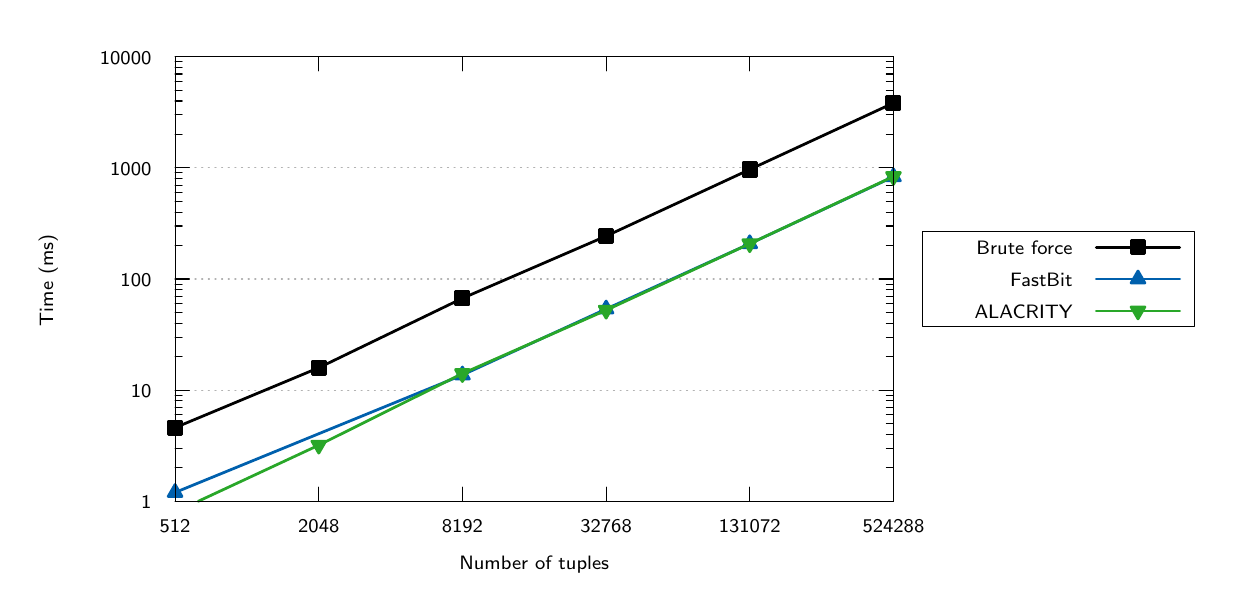
\begin{tikzpicture}[gnuplot]
%% generated with GNUPLOT 4.6p3 (Lua 5.2; terminal rev. 99, script rev. 100)
%% Wed 20 Aug 2014 10:51:25 AM CDT
\tikzset{every node/.append style={font={\sffamily \scriptsize}}}
\gpsolidlines
\path (0.000,0.000) rectangle (15.000,7.000);
\gpcolor{color=gp lt color axes}
\gpsetlinetype{gp lt axes}
\gpsetlinewidth{1.00}
\draw[gp path] (1.872,0.985)--(10.995,0.985);
\gpcolor{color=gp lt color border}
\gpsetlinetype{gp lt border}
\draw[gp path] (1.872,0.985)--(2.052,0.985);
\draw[gp path] (10.995,0.985)--(10.815,0.985);
\node[gp node right] at (1.688,0.985) { 1};
\draw[gp path] (1.872,1.410)--(1.962,1.410);
\draw[gp path] (10.995,1.410)--(10.905,1.410);
\draw[gp path] (1.872,1.658)--(1.962,1.658);
\draw[gp path] (10.995,1.658)--(10.905,1.658);
\draw[gp path] (1.872,1.835)--(1.962,1.835);
\draw[gp path] (10.995,1.835)--(10.905,1.835);
\draw[gp path] (1.872,1.972)--(1.962,1.972);
\draw[gp path] (10.995,1.972)--(10.905,1.972);
\draw[gp path] (1.872,2.083)--(1.962,2.083);
\draw[gp path] (10.995,2.083)--(10.905,2.083);
\draw[gp path] (1.872,2.178)--(1.962,2.178);
\draw[gp path] (10.995,2.178)--(10.905,2.178);
\draw[gp path] (1.872,2.260)--(1.962,2.260);
\draw[gp path] (10.995,2.260)--(10.905,2.260);
\draw[gp path] (1.872,2.332)--(1.962,2.332);
\draw[gp path] (10.995,2.332)--(10.905,2.332);
\gpcolor{color=gp lt color axes}
\gpsetlinetype{gp lt axes}
\draw[gp path] (1.872,2.397)--(10.995,2.397);
\gpcolor{color=gp lt color border}
\gpsetlinetype{gp lt border}
\draw[gp path] (1.872,2.397)--(2.052,2.397);
\draw[gp path] (10.995,2.397)--(10.815,2.397);
\node[gp node right] at (1.688,2.397) { 10};
\draw[gp path] (1.872,2.821)--(1.962,2.821);
\draw[gp path] (10.995,2.821)--(10.905,2.821);
\draw[gp path] (1.872,3.070)--(1.962,3.070);
\draw[gp path] (10.995,3.070)--(10.905,3.070);
\draw[gp path] (1.872,3.246)--(1.962,3.246);
\draw[gp path] (10.995,3.246)--(10.905,3.246);
\draw[gp path] (1.872,3.383)--(1.962,3.383);
\draw[gp path] (10.995,3.383)--(10.905,3.383);
\draw[gp path] (1.872,3.495)--(1.962,3.495);
\draw[gp path] (10.995,3.495)--(10.905,3.495);
\draw[gp path] (1.872,3.589)--(1.962,3.589);
\draw[gp path] (10.995,3.589)--(10.905,3.589);
\draw[gp path] (1.872,3.671)--(1.962,3.671);
\draw[gp path] (10.995,3.671)--(10.905,3.671);
\draw[gp path] (1.872,3.743)--(1.962,3.743);
\draw[gp path] (10.995,3.743)--(10.905,3.743);
\gpcolor{color=gp lt color axes}
\gpsetlinetype{gp lt axes}
\draw[gp path] (1.872,3.808)--(10.995,3.808);
\gpcolor{color=gp lt color border}
\gpsetlinetype{gp lt border}
\draw[gp path] (1.872,3.808)--(2.052,3.808);
\draw[gp path] (10.995,3.808)--(10.815,3.808);
\node[gp node right] at (1.688,3.808) { 100};
\draw[gp path] (1.872,4.233)--(1.962,4.233);
\draw[gp path] (10.995,4.233)--(10.905,4.233);
\draw[gp path] (1.872,4.481)--(1.962,4.481);
\draw[gp path] (10.995,4.481)--(10.905,4.481);
\draw[gp path] (1.872,4.658)--(1.962,4.658);
\draw[gp path] (10.995,4.658)--(10.905,4.658);
\draw[gp path] (1.872,4.795)--(1.962,4.795);
\draw[gp path] (10.995,4.795)--(10.905,4.795);
\draw[gp path] (1.872,4.906)--(1.962,4.906);
\draw[gp path] (10.995,4.906)--(10.905,4.906);
\draw[gp path] (1.872,5.001)--(1.962,5.001);
\draw[gp path] (10.995,5.001)--(10.905,5.001);
\draw[gp path] (1.872,5.083)--(1.962,5.083);
\draw[gp path] (10.995,5.083)--(10.905,5.083);
\draw[gp path] (1.872,5.155)--(1.962,5.155);
\draw[gp path] (10.995,5.155)--(10.905,5.155);
\gpcolor{color=gp lt color axes}
\gpsetlinetype{gp lt axes}
\draw[gp path] (1.872,5.220)--(10.995,5.220);
\gpcolor{color=gp lt color border}
\gpsetlinetype{gp lt border}
\draw[gp path] (1.872,5.220)--(2.052,5.220);
\draw[gp path] (10.995,5.220)--(10.815,5.220);
\node[gp node right] at (1.688,5.220) { 1000};
\draw[gp path] (1.872,5.644)--(1.962,5.644);
\draw[gp path] (10.995,5.644)--(10.905,5.644);
\draw[gp path] (1.872,5.893)--(1.962,5.893);
\draw[gp path] (10.995,5.893)--(10.905,5.893);
\draw[gp path] (1.872,6.069)--(1.962,6.069);
\draw[gp path] (10.995,6.069)--(10.905,6.069);
\draw[gp path] (1.872,6.206)--(1.962,6.206);
\draw[gp path] (10.995,6.206)--(10.905,6.206);
\draw[gp path] (1.872,6.318)--(1.962,6.318);
\draw[gp path] (10.995,6.318)--(10.905,6.318);
\draw[gp path] (1.872,6.412)--(1.962,6.412);
\draw[gp path] (10.995,6.412)--(10.905,6.412);
\draw[gp path] (1.872,6.494)--(1.962,6.494);
\draw[gp path] (10.995,6.494)--(10.905,6.494);
\draw[gp path] (1.872,6.566)--(1.962,6.566);
\draw[gp path] (10.995,6.566)--(10.905,6.566);
\gpcolor{color=gp lt color axes}
\gpsetlinetype{gp lt axes}
\draw[gp path] (1.872,6.631)--(10.995,6.631);
\gpcolor{color=gp lt color border}
\gpsetlinetype{gp lt border}
\draw[gp path] (1.872,6.631)--(2.052,6.631);
\draw[gp path] (10.995,6.631)--(10.815,6.631);
\node[gp node right] at (1.688,6.631) { 10000};
\draw[gp path] (1.872,0.985)--(1.872,1.165);
\draw[gp path] (1.872,6.631)--(1.872,6.451);
\node[gp node center] at (1.872,0.677) { 512};
\draw[gp path] (3.697,0.985)--(3.697,1.165);
\draw[gp path] (3.697,6.631)--(3.697,6.451);
\node[gp node center] at (3.697,0.677) { 2048};
\draw[gp path] (5.521,0.985)--(5.521,1.165);
\draw[gp path] (5.521,6.631)--(5.521,6.451);
\node[gp node center] at (5.521,0.677) { 8192};
\draw[gp path] (7.346,0.985)--(7.346,1.165);
\draw[gp path] (7.346,6.631)--(7.346,6.451);
\node[gp node center] at (7.346,0.677) { 32768};
\draw[gp path] (9.170,0.985)--(9.170,1.165);
\draw[gp path] (9.170,6.631)--(9.170,6.451);
\node[gp node center] at (9.170,0.677) { 131072};
\draw[gp path] (10.995,0.985)--(10.995,1.165);
\draw[gp path] (10.995,6.631)--(10.995,6.451);
\node[gp node center] at (10.995,0.677) { 524288};
\draw[gp path] (1.872,6.631)--(1.872,0.985)--(10.995,0.985)--(10.995,6.631)--cycle;
\node[gp node center,rotate=-270] at (0.246,3.808) {Time (ms)};
\node[gp node center] at (6.433,0.215) {Number of tuples};
\draw[gp path] (11.363,3.201)--(11.363,4.415)--(14.815,4.415)--(14.815,3.201)--cycle;
\node[gp node right] at (13.387,4.213) {Brute force};
\gpcolor{rgb color={0.000,0.000,0.000}}
\gpsetlinetype{gp lt plot 2}
\gpsetlinewidth{2.50}
\draw[gp path] (13.571,4.213)--(14.631,4.213);
\draw[gp path] (1.872,1.920)--(3.697,2.681)--(5.521,3.563)--(7.346,4.353)--(9.170,5.199)%
  --(10.995,6.043);
\gpsetpointsize{6.00}
\gppoint{gp mark 5}{(1.872,1.920)}
\gppoint{gp mark 5}{(3.697,2.681)}
\gppoint{gp mark 5}{(5.521,3.563)}
\gppoint{gp mark 5}{(7.346,4.353)}
\gppoint{gp mark 5}{(9.170,5.199)}
\gppoint{gp mark 5}{(10.995,6.043)}
\gppoint{gp mark 5}{(14.101,4.213)}
\gpcolor{color=gp lt color border}
\node[gp node right] at (13.387,3.808) {FastBit};
\gpcolor{rgb color={0.000,0.376,0.678}}
\gpsetlinetype{gp lt plot 0}
\draw[gp path] (13.571,3.808)--(14.631,3.808);
\draw[gp path] (1.872,1.097)--(5.521,2.589)--(7.346,3.427)--(9.170,4.256)--(10.995,5.106);
\gpsetpointsize{7.20}
\gppoint{gp mark 9}{(1.872,1.097)}
\gppoint{gp mark 9}{(5.521,2.589)}
\gppoint{gp mark 9}{(7.346,3.427)}
\gppoint{gp mark 9}{(9.170,4.256)}
\gppoint{gp mark 9}{(10.995,5.106)}
\gppoint{gp mark 9}{(14.101,3.808)}
\gpcolor{color=gp lt color border}
\node[gp node right] at (13.387,3.403) {ALACRITY};
\gpcolor{rgb color={0.161,0.655,0.161}}
\draw[gp path] (13.571,3.403)--(14.631,3.403);
\draw[gp path] (2.166,0.985)--(3.697,1.698)--(5.521,2.607)--(7.346,3.412)--(9.170,4.256)%
  --(10.995,5.110);
\gppoint{gp mark 11}{(3.697,1.698)}
\gppoint{gp mark 11}{(5.521,2.607)}
\gppoint{gp mark 11}{(7.346,3.412)}
\gppoint{gp mark 11}{(9.170,4.256)}
\gppoint{gp mark 11}{(10.995,5.110)}
\gppoint{gp mark 11}{(14.101,3.403)}
\gpcolor{color=gp lt color border}
\gpsetlinetype{gp lt border}
\gpsetlinewidth{1.00}
\draw[gp path] (1.872,6.631)--(1.872,0.985)--(10.995,0.985)--(10.995,6.631)--cycle;
%% coordinates of the plot area
\gpdefrectangularnode{gp plot 1}{\pgfpoint{1.872cm}{0.985cm}}{\pgfpoint{10.995cm}{6.631cm}}
\end{tikzpicture}
%% gnuplot variables

\caption{Indexing performance.}
\label{fig:indexing_perf}
\vspace{-20pt}
\end{figure}

In the future more plugins will be added, with or without external dependency
(e.g., PyTables indexing, bitmap indexing).
To satisfy that need, dynamic plugin loading and registration will be supported,
allowing external libraries to plug to the current interface.

\subsection{Limitations}

There are some existing limitations in the use of indices in the current
implementation: FastBit and ALACRITY do not support incremental updates,
an index is a shared resource for a dataset. Taken together, these conspire to
put limits on application updates to datasets with indices.
Additionally, because FastBit and ALACRITY do not allow incremental updates to
an index, each modification to an existing index forces the index to be entirely
rebuilt. The limitation in FastBit and ALACRITY will need to be addressed in
the base packages' implementation, so that incremental updates
to their index information can be made.

\subsubsection*{Questions}
Some questions are still open regarding the handling of indices:
\begin{enumerate}
%\item How could an index be built and queried in parallel for a dataset that already exists?
\item How to handle index updates when the specified index plugin is not available?
\textit{In traditional databases, stored procedures are saved with the data and
therefore available at any time, but that is not the case here.
We could mark the index as out of date and rebuild the index when the plugin is
available again.}
\item How to handle index queries when the specified index plugin is not
available? \textit{We could fallback to another plugin and do a brute force query on the data.}
\end{enumerate}

\subsection{Support for HDF5 Compound Types}

In a simple scenario, the HDF5 datatype used for creating the dataset can be defined
as a native and simple type. Therefore, building an index on this dataset implies
building that index from the entire dataset. However, in more complex scenarios, the
dataset may have been created by using a compound datatype, hence defining
multiple fields composed of native and simple datatypes within that same dataset.
Consequently, creating an index from that dataset requires the user to select a
particular field to be indexed, which may lead to having multiple indices per dataset
depending on the number of fields that it contains. This can be done by passing
the \texttt{datatype\_id} of the field to be indexed to the \texttt{xcpl\_id},
the index creation property list, of the \texttt{H5Xcreate} call, which passes
it down to the plugin \texttt{create} callback. As multiple fields can be defined,
the field \texttt{datatype\_id} must be stored along with the existing metadata, within the
\texttt{idx\_info} message (see~\FigureRef{fig:hdf5_index}) so that the index
associated to the field can be retrieved at the time of the query.
When doing a query, the compound type is passed to the \texttt{H5Qcreate} call.
The corresponding index is then used and the query is passed to the \texttt{query}
callback of the plugin.

Consequently, when removing an index, one may choose to remove the index that
corresponds to a particular field. This can be achieved by calling \texttt{H5Xget\_info},
compare the datatype returned within the info structure, and pass the index number
that needs to be removed.

\subsection{Support for HDF5 Chunking}

To support indexing of HDF5 chunks, we make each chunk a local \textit{sub-dataset}
of the original dataset. In that sense, handling every chunk can be seen as handling
a dataset from the indexing plugin point of view. If the dataset is chunked,
at the time of the index creation, we create a B-tree\footnote{The B-tree could also
be replaced by a map object.} (physically
stored on disk) that maps the coordinates of the chunks to the index plugin metadata.
When the \texttt{create} callback is called (by representing the chunk as
a local dataset, i.e., making the dataset layout point to the address of the chunk),
metadata information is returned and stored.
In the case of contiguous datasets, the index metadata as well as the index plugin ID is
stored within the dataset header of the index info message (see~\FigureRef{fig:hdf5_index}).
In the case of chunked datasets, multiple metadata that correspond to each index created
from each chunck may be accessed. Therefore, only the address of the B-tree that contains the 
metadata pieces for each chunk is stored in that header message and the index
metadata itself is stored in the B-tree.

When the dataset is opened and the index reopened, we can lookup the index
information in the B-tree that corresponds to each chunk and call the \texttt{open}
callback using the associated metadata.
%write
%   if (chunked)
%     modify I/O loop
Similarly, when a query is issued and needs to be answered, the chunks that
correspond to the selection passed to the \texttt{H5Dquery} call are selected
and their index is used to answer that query. The selection returned is then
added to a global selection, which is then in turn returned to the user.
Finally, when \texttt{H5Xremove} is called, the \texttt{delete} plugin callback is
invoked for each chunk, by using the index metadata information stored in the B-tree.

\subsection{Support for Parallel Indexing}

An important design choice to support parallel indexing is to give as much
freedom as possible to the indexing plugin developer so that in the case when
the indexing library supports parallel indexing, it is still possible to take
advantage of it. Three options are available to support parallel indexing
from the previous interface:
\begin{itemize}
\item Let the index creation be collective. This however implies having synchronization
points, which is the main constraint.
\item Let the index creation be independent. However, creating datasets to
store the index data must be done collectively\footnote{An option could be to use
the metadata server VOL plugin but this option is not easily doable yet.}.
\item Make the index creation in two phases. One that consists of
building the index in parallel, independently, and gathering the information (index size, etc)
at the end. The other that consists of letting the dataset creation be done by a master
process, which can then let the other processes write the index data independently.
There could however be a memory constraint in this case if the index data has to
be kept in memory between these two phases (though building the index twice is not
a good solution either).
\end{itemize}

Changes in the plugin interface include passing the parallel context to the
callback (MPI communicator), which can be done by using the index access property
list.
In the case of chunked datasets, one may also want to operate on several chunks
at the same time, in parallel. This can be done by passing a list of IDs that
corresponds to each chunk to the callbacks. However, this also makes the plugin
interface more heavy.

\section{HDF5 and tools}

Existing HDF5 tools must be compatible and take into account the existence of
indices in the file if there are any. For reference, the following behavior for
the tools is given:

\begin{itemize}
\item h5copy: copy
\item h5dump: report index information
\item h5ls: report index information
\item h5diff: ignore index information?
\item h5repack: copy index information / or generate index
\item h5edit: ignore index information?
\item h5toh4: ignore index information?
\item h5import: ignore index information
\end{itemize}

Additional tools for indexing data and answering queries will also be added
in the future.

\section{Usage Example}

In the following example, we show how one can make use of the query and
indexing interface to retrieve a dataspace selection within a dataset.
For simplicity's sake, we first create a dataset within the file, then open it to
create and attach a new index, in order to finally query data from it.
Note that for convenience, calls to directly read data that corresponds to the
result of the index query may be moved to the high-level API in the future.

{\lstsetc
\begin{lstlisting}
#define NTUPLES 256

int
main(int argc, char *argv[])
{
    float data[NTUPLES];
    hsize_t dims[1] = {NTUPLES};
    hid_t t file_id, dataspace_id, dataset_id;
    hid_t query_id, result_space_id;
    size_t result_npoints;
    float *result;
    int i;

    /* Initialize data. */
    for(i = 0; i < NTUPLES; i++) data[i] = (float) i;

    /* Create file. */
    file_id = H5Fcreate(file_name, H5F_ACC_TRUNC, H5P_DEFAULT, H5P_DEFAULT);

    /* Create the data space for the dataset. */
    dataspace_id = H5Screate_simple(rank, dims, NULL);

    /* Create dataset. */
    dataset_id = H5Dcreate(file_id, "Pressure", H5T_NATIVE_FLOAT, dataspace_id,
        H5P_DEFAULT, H5P_DEFAULT, H5P_DEFAULT);

    /* Write dataset. */
    H5Dwrite(dataset_id, H5T_NATIVE_FLOAT, H5S_ALL, H5S_ALL, H5P_DEFAULT, data);

    /* Close the dataset. */
    H5Dclose(dataset_id);

    /* Close dataspace. */
    H5Sclose(dataspace_id);

    /* Open dataset. */
    dataset_id = H5Dopen(file_id, "Pressure", H5P_DEFAULT);

    /* Create index using FastBit. */
    H5Xcreate(file_id, H5X_PLUGIN_FASTBIT, dataset_id, H5P_DEFAULT);

    /* Close the dataset. */
    H5Dclose(dataset_id);

    /* Create a simple query */
    query_id = H5Qcreate(H5Q_TYPE_DATA_ELEM, H5Q_MATCH_EQUAL, H5T_NATIVE_FLOAT,
        &query_value);

    /* Open dataset. */
    dataset_id = H5Dopen(file_id, "Pressure", H5P_DEFAULT);

    /* Use query to select elements in the dataset. */
    result_space_id = H5Dquery(dataset_id, query_id);

    /* Allocate space to read data. */ 
    result_npoints = (size_t) H5Sget_select_npoints(result_space_id);
    result = malloc(result_npoints * sizeof(float));

    /* Read data using result_space_id. */
    H5Dread(dataset_id, H5T_NATIVE_FLOAT, H5S_ALL, result_space_id,
        H5P_DEFAULT, result);

    /* Use result. */

    /* Free result. */
    free(result);

    /* Close the dataset. */
    H5Dclose(dataset_id);

    /* Close dataspace. */
    H5Sclose(result_space_id);

    /* Close query. */
    H5Qclose(query_id);

    /* Close the file. */
    H5Fclose(file_id);
}
\end{lstlisting}
}

%\section{Conclusion}
%Document in progress.



\section*{Revision History}
\makerevisions

%% References
\bibliographystyle{abbrv}
\bibliography{analysis_ext}

\end{document}
